\documentclass[a4paper,12pt]{article}

\usepackage[T2A]{fontenc}			
\usepackage[utf8]{inputenc}			
\usepackage[english,russian]{babel}	

\usepackage[
bookmarks=true, colorlinks=true, unicode=true,
urlcolor=black,linkcolor=black, anchorcolor=black,
citecolor=black, menucolor=black, filecolor=black,
]{hyperref}

\usepackage{color}
\usepackage{caption}
\DeclareCaptionFont{white}{\color{black}}
\DeclareCaptionFormat{listing}{\colorbox{white}{\parbox{\textwidth}{#1#2#3}}}
\captionsetup[lstlisting]{format=listing,labelfont=white,textfont=white}

\usepackage{amsmath,amsfonts,amssymb,amsthm,mathtools} 
\usepackage{wasysym}

\usepackage{graphicx}
%\usepackage[cache=false]{minted}
\usepackage{cmap}
\usepackage{indentfirst}

\usepackage{listings} 
\usepackage{fancyvrb}

\usepackage{geometry}
\geometry{left=2cm}
\geometry{right=1.5cm}
\geometry{top=1cm}
\geometry{bottom=2cm}

\setlength{\parindent}{5ex}
\setlength{\parskip}{0.5em}

\usepackage{pgfplots}
\usepackage{longtable}

\begin{document}
	\lstset{ %
		language=C,                 % выбор языка для подсветки (здесь это С)
		basicstyle=\small\sffamily, % размер и начертание шрифта для подсветки кода
		numbers=left,               % где поставить нумерацию строк (слева\справа)
		numberstyle=\tiny,           % размер шрифта для номеров строк
		stepnumber=1,                   % размер шага между двумя номерами строк
		numbersep=5pt,                % как далеко отстоят номера строк от подсвечиваемого кода
		backgroundcolor=\color{white}, % цвет фона подсветки - используем \usepackage{color}
		showspaces=false,            % показывать или нет пробелы специальными отступами
		showstringspaces=false,      % показывать или нет пробелы в строках
		showtabs=false,             % показывать или нет табуляцию в строках
		frame=single,              % рисовать рамку вокруг кода
		tabsize=2,                 % размер табуляции по умолчанию равен 2 пробелам
		captionpos=t,              % позиция заголовка вверху [t] или внизу [b] 
		breaklines=true,           % автоматически переносить строки (да\нет)
		breakatwhitespace=false, % переносить строки только если есть пробел
		escapeinside={\%*}{*)}   % если нужно добавить комментарии в коде
	}
	
	% Титульный лист
	\begin{figure}[h!]
		\begin{center}
			{
\includegraphics[scale = 0.4]{titul.jpg}}
			\label{titul}
		\end{center}
	\end{figure}
	
	\vspace*{15mm} 
	
	\huge
	\begin{center}
		Дисциплина: <<Моделирование>>
	\end{center}
	
	\begin{center}
		Лабораторная работа №2
	\end{center}

	
	\huge
	\begin{center}
		Тема работы:\\
		<<Изучение функций и плотностей распределения заданных случайных величин>>
	\end{center}
	\vspace*{25mm} 
	
	\large
	\begin{flushright}
		Студент: Левушкин И. К. \\
		Группа: ИУ7-72Б \\
		Преподаватель: Рудаков И. В. \\
	\end{flushright}
	
	\vspace*{25mm}
	\begin{center}
		Москва, 2020 г.  
	\end{center}
	\thispagestyle{empty}
	
	
	\newpage
	
	\section*{Задание}
	
	Реализовать программу для построения графиков функции и плотности распределения для равнмерного и пуассоновского разпределений.
	
	\section*{Формализация}
	
	\subsection*{Равномерное распределение}
	
	Равномерным распределением непрерывной случайной величины называется распределение, в котором значения случайной величины с двух сторон ограничены и в границах интервала имеют одинаковую вероятность.
	
	Функция распределения:
	
	\[
	F(x) = \begin{cases}
	0, \text{если} x < a,\\
	\frac{x-a}{b-a}, \text{если} x \in [a, b],\\
	1, \text{если} x > b.\\
	\end{cases}
	\]
	
	
	Плотность распределения:
	
	\[
	f(x) = \begin{cases}
	\frac{1}{b-a}, \text{если } x \in [a, b],\\
	0, \text{если } x \notin [a, b].\\
	\end{cases}
	\]
	
	\subsection*{Пуассоновское распределение}
	
	Распределение Пуассона — распределение дискретного типа случайной величины, представляющей собой число событий, произошедших за фиксированное время, при условии, что данные события происходят с некоторой фиксированной средней интенсивностью и независимо друг от друга.
	
	Функция вероятности:
	
	\[
	P_k(\lambda) = \frac{\lambda^k e^{-\lambda}}{k!}
	\]
	
	Функция распределения:
	
	\[
	F(x) = \sum_{k=0}^{N} \frac{\lambda^k e^{-\lambda}}{k!}
	\]
	
	
	\section*{Результаты работы}
	
	\subsection*{Равномерное распределение}
	
	Ниже приведены графики функции распределения и плотности распределения равномерного распределения с параметрами $a = -1, b = 1$ на интервале $[-2.0; 2.0]$:
	
	\begin{figure}[h!]
		\begin{minipage}[b]{0.5\textwidth}
			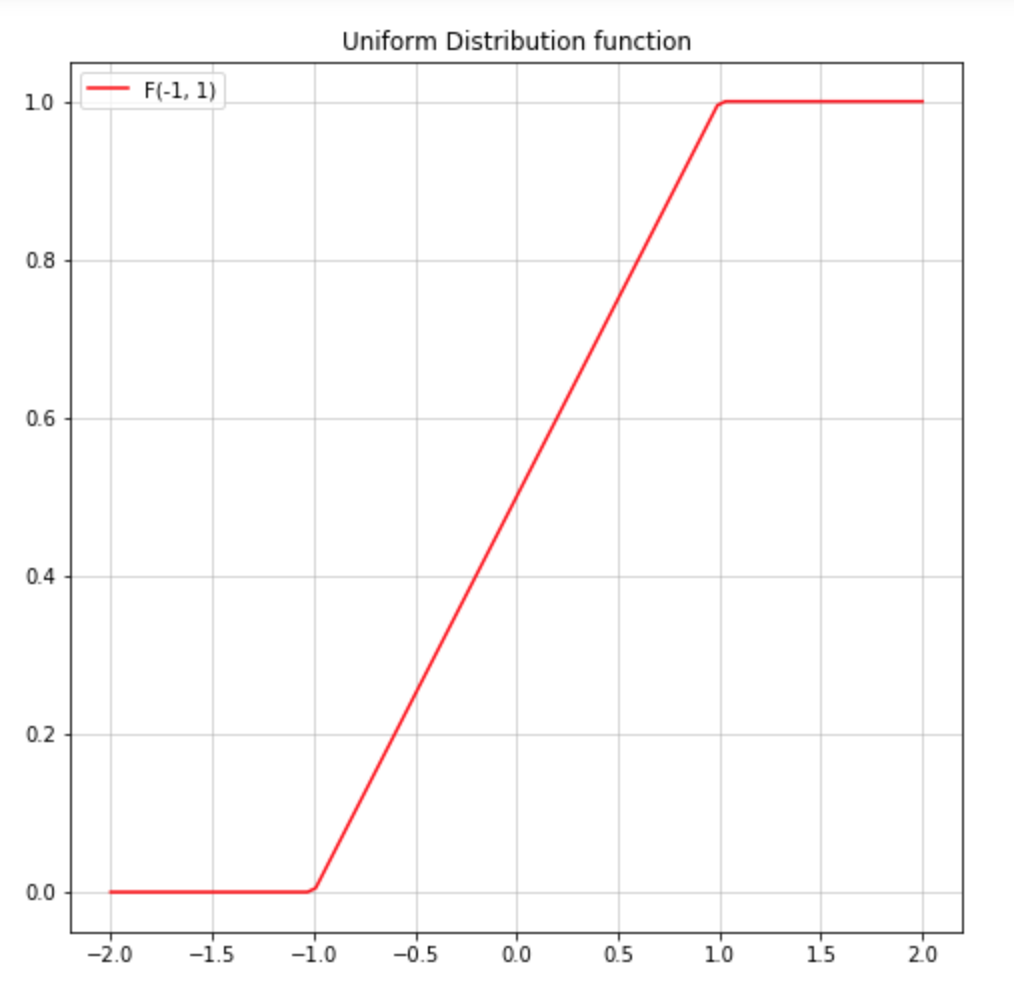
\includegraphics[width=\textwidth]{examples/F_uniform.png}
			\center{Функция распределения равномерного распределения}
		\end{minipage}
		\begin{minipage}[b]{0.5\textwidth}
			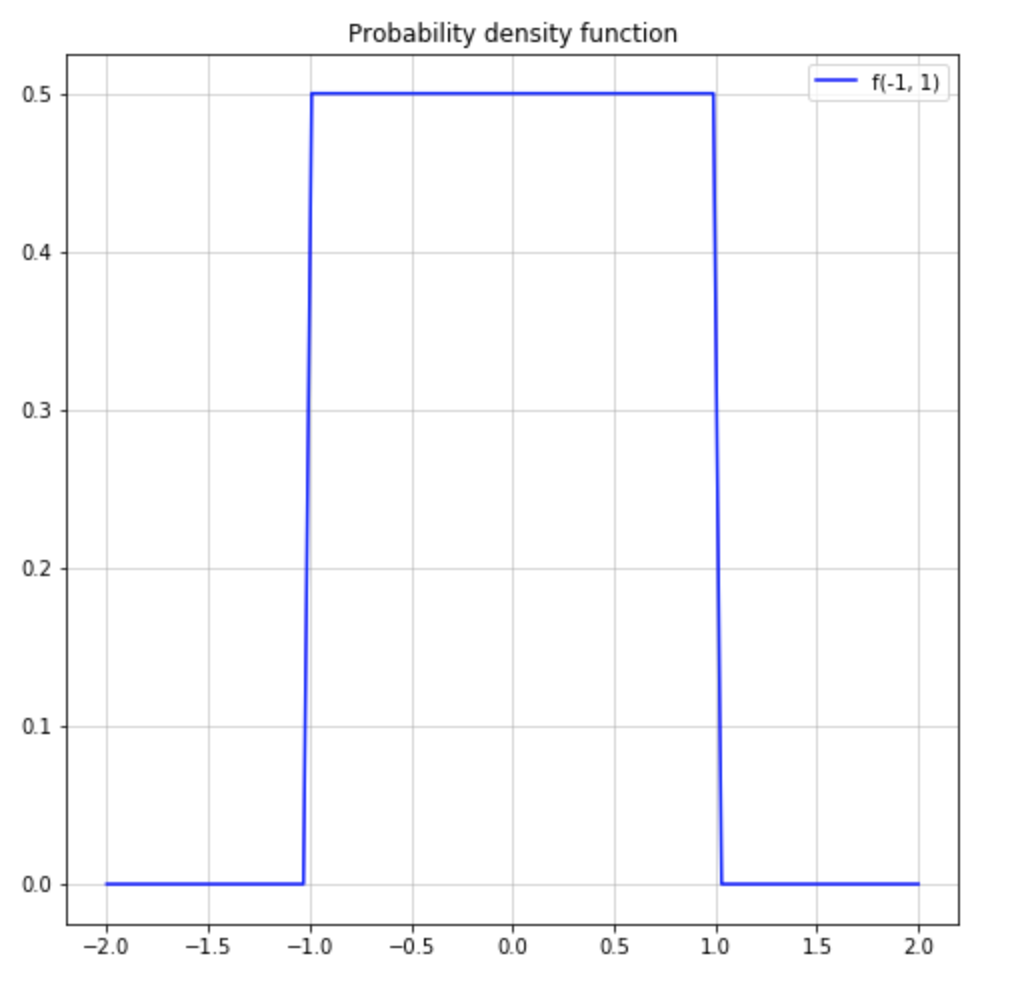
\includegraphics[width=\textwidth]{examples/f_uniform2.png}
			\center{Плотность распределения равномерного распределения}
		\end{minipage}
		\label{ris:examples_1_2}
	\end{figure}

	\newpage

	\subsection*{Пуассоновское распределение}
	
	Ниже приведены графики функции распределения и функции вероятности Пуассоновского распределения с параметром $\lambda = 10$ на интервале $[0.0; 20.0]$:
	
	\begin{figure}[h!]
		\begin{minipage}[b]{0.5\textwidth}
			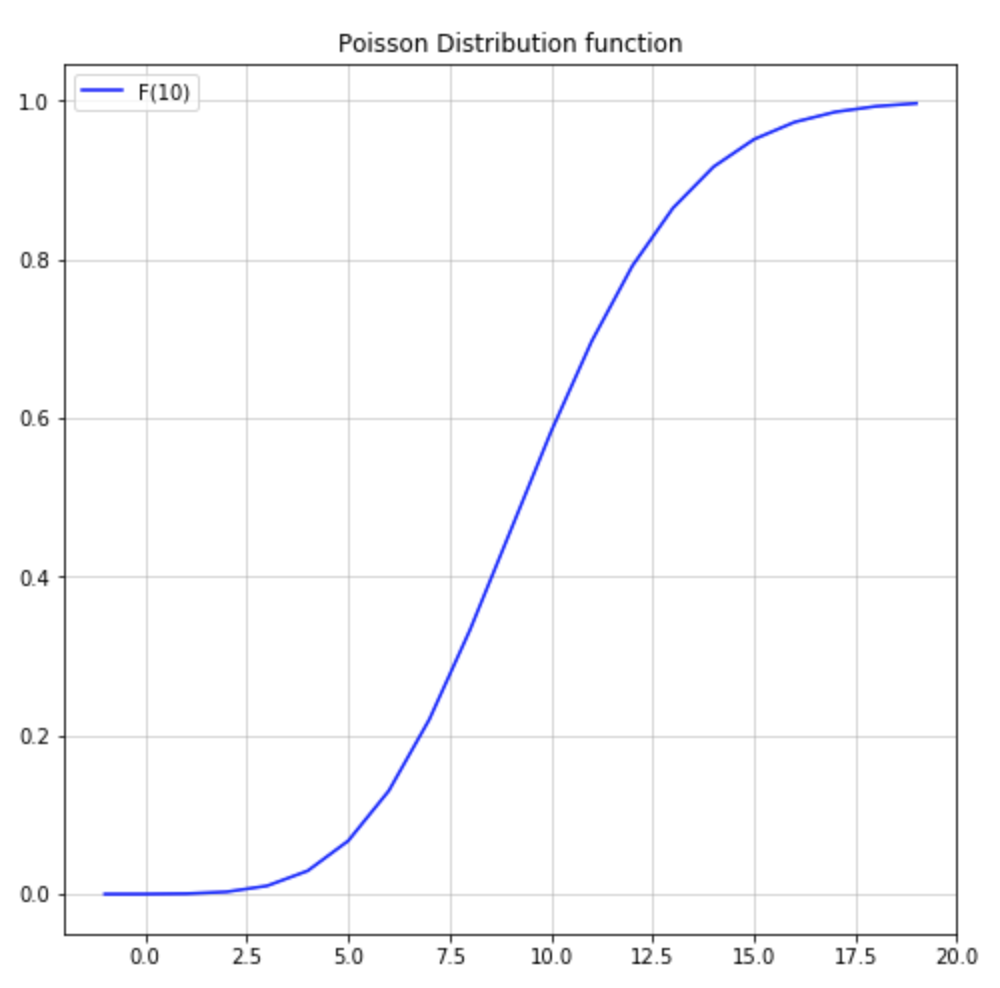
\includegraphics[width=\textwidth]{examples/F_puass.png}
			\center{Функция распределения Пуассоновского распределения}
		\end{minipage}
		\begin{minipage}[b]{0.5\textwidth}
			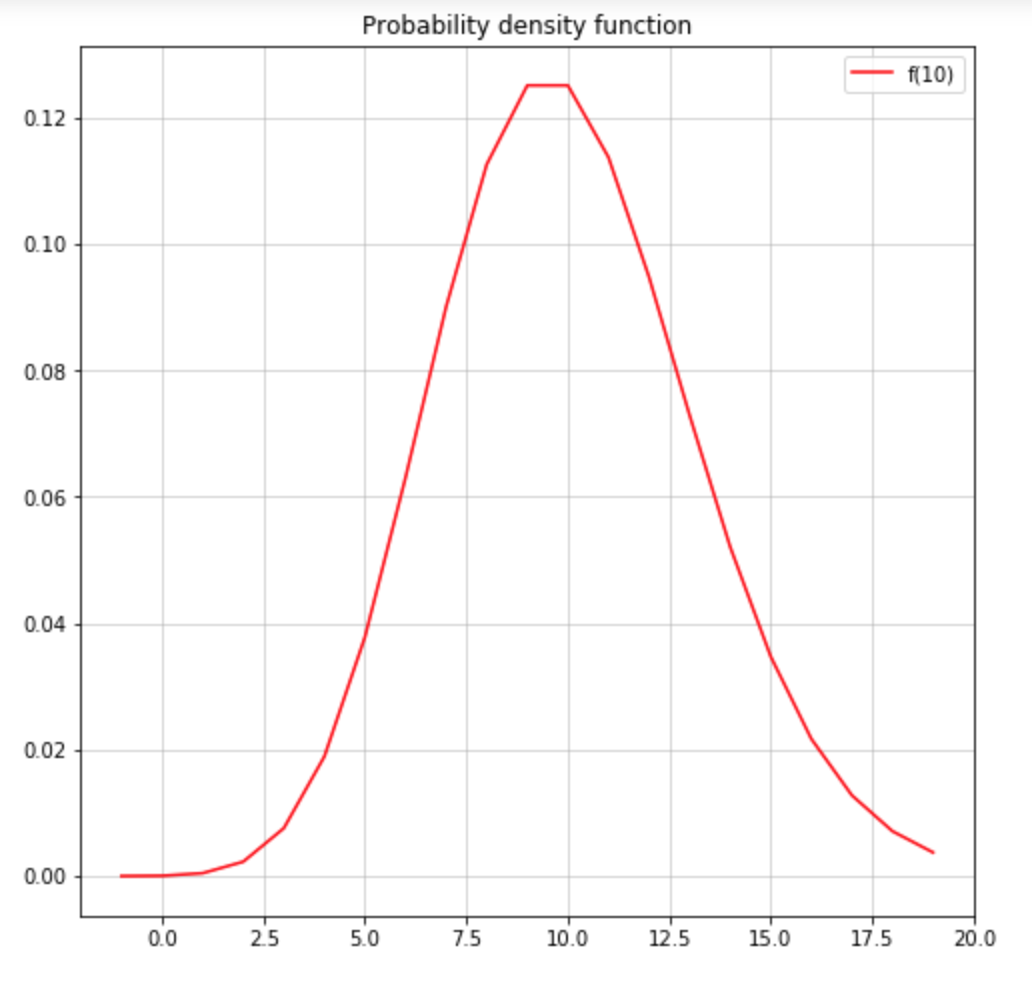
\includegraphics[width=\textwidth]{examples/p_puass.png}
			\center{Функция вероятности Пуассоновского распределения}
		\end{minipage}
		\label{ris:examples_3_4}
	\end{figure}
	
	\section*{Вывод}
	
	Исходя из приведенных результатов работы можно сделать вывод, что графики распределений полностью соответствуют определениям, описанным в разделе формализации задачи. А именно:
	
	\begin{itemize}
		\item При равномерном распределении плотность распределения имеет одинаковую вероятность $p = 0.5$ на интервале $[-1, 1]$,
		\item При Пуассоновском распределении функция вероятности принимает наибольшее значение при заданном параметре $\lambda = 10$.
	\end{itemize}
	
\end{document}